\documentclass[12pt]{article}
\usepackage{fullpage}
\usepackage{graphicx}
\usepackage[utf8]{inputenc}
\usepackage{amsmath}
\usepackage{graphics}
\usepackage{xcolor}
\usepackage{listings}
\usepackage{adjustbox}
\usepackage{tikz}
\usepackage[margin=1in]{geometry}
\usepackage{wasysym}
\usetikzlibrary{positioning}
\usetikzlibrary{calc,shapes, arrows, positioning, shapes.gates.ee, trees}
\usepackage{hyperref}

	\begin{document}
\begin{titlepage}

	\begin{center}
		
		
\includegraphics[width=0.3\textwidth]{UoN_Logo.png}\\
		
		THE UNIVERSITY OF NAIROBI\\
		FACULTY OF SCIENCE AND TECHNOLOGY\\
		DEPARTMENT OF MATHEMATICS\\
		\vspace{0.5cm}
	\underline{	STA : 420 PROJECT IN STATISTICS}
		\vspace{1cm}
		
\underline{	\textbf{MULTIPLE GROUP- CONFIRMATORY FACTOR ANALYSIS}}
		
		\vspace{0.5cm}
		BY:\\
		
		WAMBUA CHARLES             : \hspace{0.2cm}     I63/4248/2019\\
		\vspace{0.5cm}
		BEVERLY KIND               : \hspace{0.2cm}    I63/4240/2019\\
		\vspace{0.5cm}
		ODHIAMBO KENNEDY           : \hspace{0.2cm}    I63/4282/2019\\
		\vspace{0.5cm}
		NYAENYA DOMINIC            : \hspace{0.2cm}    I63/4261/2019\\
		\vspace{0.5cm}
		DOKTA PETER                : \hspace{0.2cm}    I63/136668/2019\\
		\vspace{0.5cm}
		\textbf{SUPERVISOR:}\\
		\vspace{0.5cm}
		DR. LYDIA ADHIAMBO MUSIGA
		
		\vspace{3cm}
		
		
		APRIL 2023
	
		
	\end{center}
\end{titlepage}

\textbf{Chapter 2}
\section{LITERATURE REVIEW}
In this chapter, we review the existing research and scholarship related to mental health and its effects on a person’s productivity as well as the interaction between an individual’s cognitive, affective and somatic symptoms of depression. A description of this consensus inevitably leads to a set of core issues that must be addressed if psychiatric scientists are to establish a more adequate explanation of mental health assessment and procedures. Several questions need to be answered with respect to; How an individual and environment contribute to a person’s mental health? How does mental health affect productivity at workplaces as well as learning institutions? How does mental health vary across age groups with the changing world of internet error post-COVID-19? What research methods are available for addressing these issues in research? The study begins with some key concepts from previous research perspectives that have contributed to recent advances in mental health understanding and then presents the implications of this knowledge for accurate screening of major depressive disorder.

In a research done by Martin et al. (2009) investigated whether different types of health promotion intervention in the workplace reduce depression and anxiety symptoms. A systematic review and meta-analysis were undertaken on workplace health promotion published during the period 1997-2007.Studies were considered eligible for inclusion if they evaluated the impact of an intervention using a valid indicator or specific measure of depression or anxiety symptoms. The standardized mean difference was calculated for each of the following three types of outcome measures; depression, anxiety and composite mental health. Altogether,22 studies were found that met the inclusion criteria, with a total sample size of 3409 employees post intervention, and 17 of these studies were included in the meta-analysis representing 20 intervention- control comparisons. The pooled results indicated small but positive overall effects of the interventions with respect to symptoms of depression and anxiety, but no effect on composite mental health measures. The interventions that included a direct focus on mental health had a comparable effect on depression and anxiety symptoms as did the interventions with an indirect focus on risk factors. When the aim to reduce symptoms of depression and anxiety in employee populations, a broad range of health promotion interventions appear to be effective, although the effect is small.\\

Gagan Jain et al (2013) examined the burden of depression on work productivity in the US workforce and used Patient Health Questionnaire for depression severity, the Health and Work Performance Questionnaire and Work Productivity and Activity Impairment (WPAI) Questionnaire for absenteeism and presenteeism in 1051 full-time employees for a period of three years. All levels of depression were associated with decreased work productivity and presenteeism was positively associated with severity of depression as well absenteeism which was significantly positively associated with severity of depression using the WPAI. The study showed that decreased overall productivity at all levels of depression and as severity increased, presenteeism and absenteeism worsened. \\

In another study J. Greg Serpa et al (2014), investigated major problems among Veterans specifically anxiety, depression and suicidal ideation and used pre and post Mindfulness-based Stress Reduction questionnaires to collect data on 79 veterans at an urban Veterans Health Administration medical facility and also conducted a meditation analysis to determine whether changes in mindfulness were related to changes in the other outcomes for a period of 9 weekly sessions. This led to significant reductions in anxiety, depressions, and suicidal ideation after MBSR training, improved mental health functioning scores although pain intensity and physical health functionality did not indicate improvements. The study showed that completing an MBSR program can improve symptoms of anxiety, depression and reduced suicidal ideations on health of patients. \\

In the changing world, there is a need to assess workplace health culture using evidence-based measures. In a research done by Laing and Jones,(2016), indicated that previous studies using employee level culture of health measures observed that culture of health is associated with higher levels of job satisfaction and retention [15], work engagement [16], and healthy behaviors such as physical activity and healthy eating [20]. A 2016 on US government employees (n = 4703) found that workplace culture of health was negatively correlated with anxiety and depression [21]. Similar results were observed in employees in China, where higher ratings of workplace culture of health were associated with better psychological wellbeing [22]. 
Domains of workplace culture of health such as leadership and coworkers support have been found to decrease employee health risk [8] and promote positive health behaviors [20]. However, there is only one U.S.-based study that has examined workplace health culture and emotional wellbeing from employees' perspective [21].  Other studies in this area have measured workplace culture of health from the employer-level, which may not capture a comprehensive perspective [18,19]. In addition, that study did not use a validated research tool to measure workplace culture of health, limiting its generalizability [21]. There is a need to assess workplace health culture using evidence-based measures. 

Another study was done by Magtibay et al. (2017) to to assess efficacy of blended learning to decrease stress and burnout among nurses through use of the Stress Management and Resiliency Training (SMART) program. It was assumed that Job-related stress in nurses leads to high rates of burnout, compromises patient care, and costs US healthcare organizations billions of dollars annually. Many mindfulness and resiliency programs are taught in a format that limits nurses’ attendance. Consistent with blended learning, participants chose the format that met their learning styles and goals; Web-based, independent reading, facilitated discussions. The end points of mindfulness, resilience, anxiety, stress, happiness, and burnout were measured at baseline, postintervention, and 3-month follow-up to examine within-group differences.Findings showed statistically significant, clinically meaningful decreases in anxiety, stress, and burnout and increases in resilience, happiness, and mindfulness. Results support blended learning using SMART as a strategy to increase access to resiliency training for nursing staff.

In recent years, mental health has widely been recognized as the prevalence of mental health disorders continues to rise. In this regard there has been need to come up with screening techniques to ensure accurate and effective screening tools for mental health disorders. PHQ-9 is one the tools that have been employed over time to screen severity of depression. Patient Health Questionnaire (PHQ-9) is a brief, self-administered screening tool that is commonly used to diagnose and assess the severity of depression. The questionnaire consists of nine items that correspond to the nine DSM-5 criteria for major depressive disorder. Each item asks the patient to rate the frequency of a particular symptom over the past two weeks on a scale from 0 (not at all) to 3 (nearly every day). The scores are then summed to give a total score that ranges from 0 to 27, with higher scores indicating greater severity of depression. 
Levis et al. (2019), evaluates the accuracy of the Patient Health Questionnaire-9 (PHQ-9) for screening major depression in adults using individual participant data meta-analysis. The study, which involved the DEPRESSD Collaboration, analyzed data from 27 studies, with a total of 50,788 participants. The research found that a cut-off score of 10 or above can be used regardless of age, and the PHQ-9 is similarly sensitive but may be less specific for younger patients than for older patients. The study also found that the PHQ-9 sensitivity compared with semi structured diagnostic interviews was greater than in previous conventional meta-analyses that combined reference standards and suggest that future research on the PHQ-9 should ideally be based on semi structured diagnostic interviews and should consider estimating probabilities of depression across the full spectrum of PHQ-9 screening scores, and should combine screening scores with individual characteristics to generate individualized probabilities of major depression. The research developed a web-based tool to estimate the expected number of positive screens and true and false screening outcomes based on the study's results. However, in primary care, approximately half of patients with positive screens would be false positives if this was used in practice

Leung et al.(2020) aims to evaluate the factor structure, reliability, and construct validity of the Patient Health Questionnaire-9 (PHQ-9) in a community sample of Chinese adolescents. Confirmatory factor analysis was used to examine the one-factor structure of the PHQ-9, and multiple-group CFAs were performed to test for measurement invariance across gender and age subgroups. Internal consistency reliability was evaluated using Cronbach alpha, and construct validity was assessed using Pearson correlation coefficients between PHQ-9 scores and relevant measures. The results indicate that the PHQ-9 has a one-factor structure, good reliability, and construct validity in Chinese adolescents, and it is measurement invariant across gender and age subgroups. The study's limitations include the lack of test-retest reliability evaluation and generalizability to other cultural contexts. These findings provide important information on the psychometric properties of the PHQ-9 for assessing adolescent depression and screening, highlighting the need for further research on its predictive power and generalizability.

In a more recent study, Jama et al.(2020) a meta-analysis of 44 studies was conducted to compare the sensitivity and specificity of the PHQ-2 and PHQ-9 combination with the full PHQ-9 for all participants. The study found that the sensitivity of the combination of PHQ-2 and PHQ-9 was not significantly different from the full PHQ-9, but the specificity was minimally, yet significantly higher. The study suggests that misclassifying significant depression among participants with subthreshold depressive symptoms based on fully structured interviews might explain the lower sensitivity compared with semi-structured interviews. The PHQ-2 alone had lower sensitivity or specificity, depending on the cutoff score, compared to the PHQ-9. The study concludeD that using PHQ-9 by itself may be adequate for depression screening. Jama et al.,(2020) provides valuable insights into the use of the PHQ-9 for depression screening and highlights the importance of considering the type of interview used when interpreting the results. The existence of the gap to fully explore the relationship between an individual's cognitive, affective and somatic symptoms of depression, decision to advance the research has been put into consideration. Different methods of CFA have been used to analyze and investigate if there is existence of any kind. In our research, multiple group confirmatory factor analysis is the key interest in observing this relationship.
\newpage
\textbf{Chapter 3}
\section{THEORY OF CONFIRMATORY FACTOR ANALYSIS}
\subsection{Introduction}
In this chapter, we discuss the CFA model, Invariance measurement, research approach, the procedures used to obtain the data, methods used to analyze the data and the models used.

\subsection{Conceptual Introduction to Confirmatory Factor Analysis}

Confirmatory factor analysis (CFA) is a type of structural equation (SEM) that deals specifically with measurement models, that is, the relationship between observed measures or indicators (e.g test items, test scores, behavioral observation ratings) and latent variable or factor. CFA, unlike its counterpart, exploratory factor analysis, all its aspects must be pre-specified. Therefore, it is required that the researcher has a firm prior idea, based on the pre-existing evidence and theory, of
number of factors in the data. In CFA, instead of letting the data tell us the factor structure, we pre-determine the factor structure and verify the psychometric structure of previously developed scale. CFA became more popular after a breakthrough in both computing technology on an estimation method developed by Joreskog (1969) ((Brown and Moore, 2012).
\subsubsection{Characteristics of CFA Model}
\begin{enumerate}
\item Each indicator is continuous with two causes—a single factor that the indicator is supposed to measure and all unique sources of influence represented by the error term.
\item The error terms are independent of each other and of the factors.
\item All associations are linear and the factors covary. This is why the symbol for an unanalyzed association in \ref{fig:Figure 3.1} is depicted as solid instead of dashed.
\end{enumerate}
\subsubsection{Advantages of CFA}
\begin{enumerate}
	\item CFA unlike EFA allows for the specification of relationships among the indicator uniqueness (error variances), which may have substantive importance (e.g. correlated errors due to method effects)
	\item CFA offers a very strong analytic framework for evaluating the equivalence of measurement models across distinct groups. This is accomplished by multiple group solutions or MIMIC models.
	\item CFA has the ability to estimate the relationships among variables adjusting for measurement error
\end{enumerate}

\subsubsection{Assumptions of CFA models}
\begin{enumerate}
	\item Multivariate normality (i.e the univariate distributions and the joint distribution of all variable combinations are normal)(Kline,2006)\\
	\underline{note}\\
	Violations of this assumption can lead to a distortion of goodness fit model related to the model as a whole.
	\item sufficient sample size($\geq$ 200)
	\item Correct a priori model specification
	\item Data must come from a random sample
\end{enumerate}
\subsection{The Confirmatory Factor Analysis Models}
\subsubsection{The single factor analysis model}
This focus on model identification and model fit. The single item factor analysis model is defined as
\begin{equation*}
	y_1=\tau_1 +\lambda_1 \eta + \epsilon_1
\end{equation*}
which is essentially a linear regrestion model with main predictor he factor, being latent or unobserved. $\tau$ is the intercept of the first item, $\lambda_1$ is the factor loading also termed as regression weight of the factor of the first item. $\epsilon_1$ is the residual(error) for the first item.\\
For a k common factor(s) the CFA model is;\\
\begin{center}
	\[
\left(
\begin{matrix}
	y_1= \lambda_{11}\eta_1 +...+\lambda_{1k}\eta_k +\epsilon_1 \\
	y_2= \lambda_{21}\eta_1 +...+\lambda_{2k}\eta_k +\epsilon_2 \\
	y_3 = \lambda_{31}\eta_1+...+\lambda_{3k}\eta_k +\epsilon_3 \\
	                .                  .              .      \\
	                .                  .               .     \\
	                .                  .              .     \\
	y_p=\lambda_{p1}\tau_1+...+\lambda_{pk}\tau_k +\epsilon_p \\                
	
\end{matrix}
\right)
\]
\end{center}
Which in matrix notation that the form(Johnson,2007 \& UCLA,)\\

	\begin{equation*}
	\left(
	\begin{matrix}
		y_1\\
		y_2\\
		\vdots \\
		y_p\\
	\end{matrix}
	\right) = 
	\left(\begin{matrix}
		\lambda_{11}\eta_1 & .&.&.& \lambda_{1k}\\
		\lambda_{21}\eta_1 &  .&.&. & \lambda_{2k}\\
		\vdots\\
		\lambda_{p1}\eta_1  & .&.&. &\lambda_{pk}\\
	\end{matrix}\right) \times
	\left(\begin{matrix}
		\eta_1\\
		\eta_2\\
		\vdots\\
		\eta_k\\
	\end{matrix}\right)+ \left(\begin{matrix}
		\epsilon_1\\
		\epsilon_2\\
		\vdots\\
		\epsilon_p\\
	\end{matrix}\right)
\end{equation*}

\begin{equation*}
	Y=\Lambda\eta_i + \epsilon_i
\end{equation*}
Where;
\begin{enumerate}

\item Y- is p $\times$1 vector of the observable random variables
\item $\Lambda$ is the matrix factor loading
\item $\eta_i$ refers to the k$\times$1 of the latent(unobservable) variables.
\item $\epsilon_i$ is a p$\times$1 vector of the residual(errors)
\end{enumerate}

The second equation above looks like a multiple regration model of Y on $\eta$ but it's not testable since the factors $\eta_i$ are unobserved. This model implies a particular form of variance-covariance matrix $\sum$ which is testable.

\subsubsection{Two-Factor CFA model}
Results from the one-factor CFA suggest that a one solution may capture much variance in the observed variables, however the model fit suggests that this model can be improved.
Two factor CFA model assumes;
\begin{enumerate}
	\item Factors are uncorrelated.
	\item Factors are correlated.
\end{enumerate}
\title*\textbf{{Uncorrelated factors}}\\
Proceeding with a two-factor CFA, we assume uncorrelated (or orthogonal) factors. Having a two-item factor presents a special problem for identification. In order to identify a two-item factor there are two options:
\begin{enumerate}
	\item  Freely estimate the loadings of the two items on the same factor but equate them to be equal while setting the variance of the factor at 1.
	\item Freely estimate the variance of the factor, using the marker method for the first item, but covary (correlate) the two-item factor with another factor.
\end{enumerate}
\title*\textbf{{Correlated factors}}\\
We still have the issue of that two-item factor.in model identification we can either equate the loadings and set the variance to 1 or we can covary the two-item factor with another factor and use the marker method.
\newpage
\subsection{The General CFA Model}
All models in the CFA contain factor variance, unique variance and factor loadings.\\
The factor loadings are the regression slopes for predicting the latent factor.\\
The factor variance expresses sample variability or dispersion of the factor, that is, the extent to which sample participants relative standing on the latent dimension is similar or different. \\
Unique variance or error variance is typically the unwxplained variation or simply the measurement error.\\
As an illustration we can represent CFA model as shown in the \ref{fig:Figure 3.1} below;
\begin{figure}[h]
	\centering
	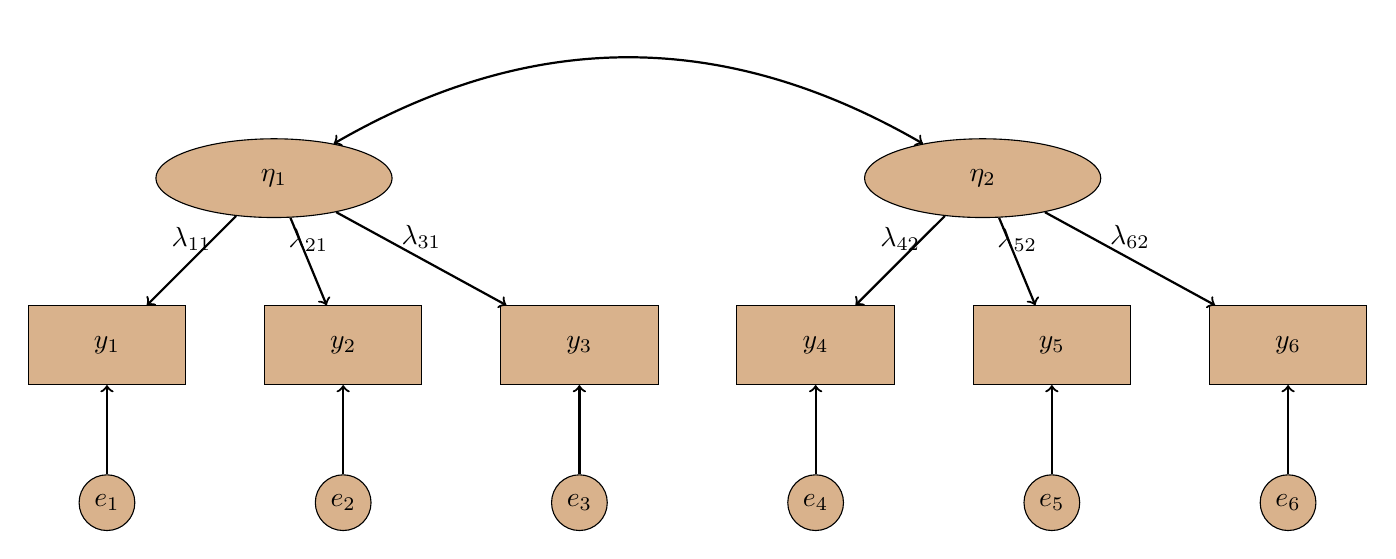
\begin{tikzpicture}[ factor/.style={draw,fill=brown!60, ellipse,minimum height=1cm, minimum width=3cm, node distance= {9cm}},
		latent/.style={draw,fill=brown!60, rectangle, minimum width=2cm, minimum height=1cm, node distance= {3cm}},
		residual/.style={draw,fill=brown!60,  circle, node distance= {2cm}}
		]
		\node [factor](x1) {$\eta_1$};
		\node [factor](x2)[right of =x1] {$\eta_2$};
		\node [latent](y1) [below left of=x1] {$y_1$};
		\node [latent](y2) [right of=y1] {$y_2$};
		\node [latent](y3) [right of=y2] {$y_3$};
		\node [latent](y4) [right of =y3] {$y_4$};
		\node [latent](y5) [right of=y4] {$y_5$};
		\node [latent](y6) [right of=y5] {$y_6$};
		\node [residual](e1) [below of=y1] {$e_1$};
		\node [residual](e2) [below of=y2] {$e_2$};
		\node [residual](e3) [below of=y3] {$e_3$};
		\node [residual](e4) [below of=y4] {$e_4$};
		\node [residual](e5) [below of=y5] {$e_5$};
		\node [residual](e6) [below of=y6] {$e_6$};
		
		\draw[thick, black, ->](x1) -- (y1) node[midway, above] {$\lambda_{11}$};
		\draw[thick, black, ->] (x1) -- (y2) node[midway, above] {$\lambda_{21}$};
		\draw[thick, black, ->] (x1) -- (y3) node[midway, above] {$\lambda_{31}$};
		\draw[thick, black, ->] (x2) -- (y4) node[midway, above] {$\lambda_{42}$};
		\draw[thick, black, ->] (x2) -- (y5) node[midway, above] {$\lambda_{52}$};
		\draw[thick, black, ->] (x2) -- (y6) node[midway, above] {$\lambda_{62}$};
		\draw[thick, black, ->] (e1) -- (y1);
		\draw[thick, black, ->] (e2) -- (y2);
		\draw[thick, black, ->] (e3) -- (y3);
		\draw[thick, black, ->] (e4) -- (y4);
		\draw[thick, black, ->] (e5) -- (y5);
		\draw[thick, black, ->] (e6) -- (y6);
		\draw[thick, black, <->] (x1) edge[bend left=30] node[above] {} (x2);
	\end{tikzpicture}
	\caption{ \textbf{Two factor CFA model with no error covariance}}
	\label{fig:Figure 3.1}
\end{figure}\\
Where $\lambda_i$ is factor loading; $e_i$ for i= 1,.., 6 is the error variance. The covariate line $\eta_1$.$\eta_2$ is the factor variance covariance.\\
This model tell us that instead of letting a relationship to exist between $\eta_1$ and $Y_4$, $Y_5$ and $Y_6$, and $\eta_2$ and $Y_1$, $Y_2$ and $Y_3$, we constrain those parameters that mesure the relationship between two sets to zero.\\
Due to parameter restriction, CFA is also referred to as restricted factor model. The factor loading is fixed to zero for the indicator that do not measure the factor. Fixing the parameters over identifies the model and this gives us more degrees of freedom in our model which in turn enables us to test model fit of our model as compared to matrix that we observed as simple variance covariance matrix.

\subsubsection{The Fundamental Equation of CFA Model}
The CFA model uses the model implied covariance matrix defined as;

\begin{equation}
	\sum(\theta)= Cov(y)= \Lambda \Psi\Lambda'+\Theta_\epsilon \label{eq:3.1}
\end{equation}
Where\\
$\Lambda$ is a matrix of factor loading\\
$\Psi$ is the variance-covariance matrix of latent variables\\
$\Theta_\epsilon$ is the Variance-covariance of residual errors\\

As an illustration, consider a two factor CFA model \ref{fig:Figure 3.2} below;

\begin{figure}[h]
	\centering
	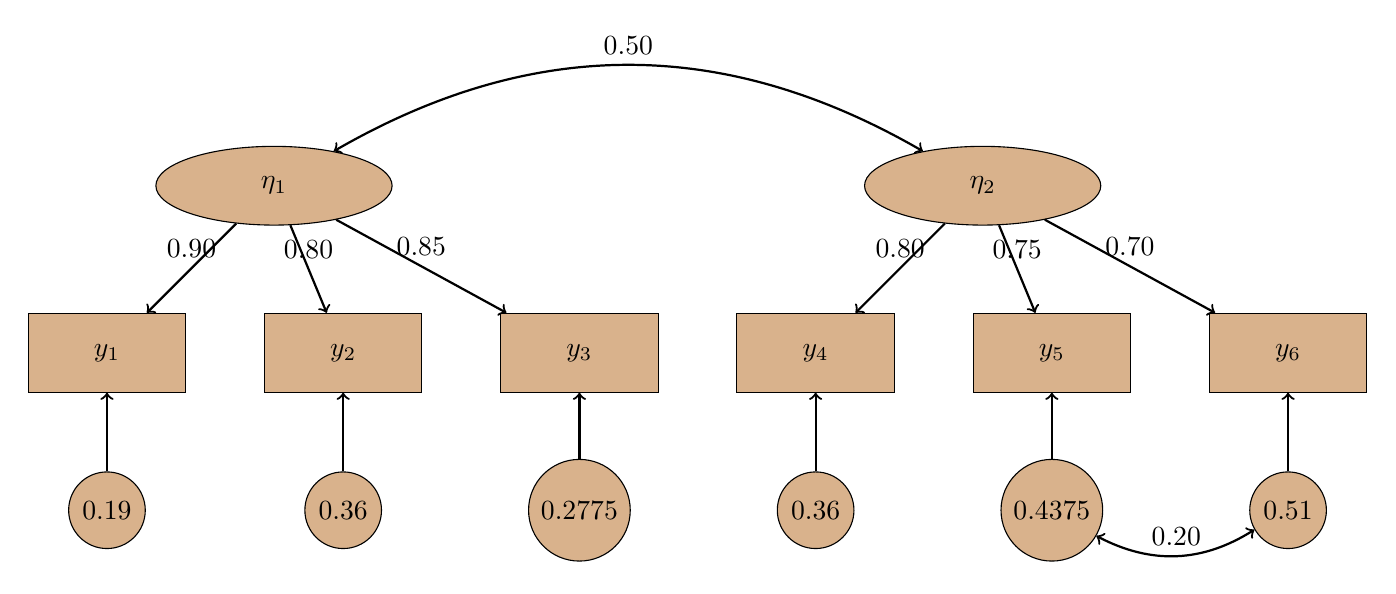
\begin{tikzpicture}[ factor/.style={draw,fill=brown!60, ellipse,minimum height=1cm, minimum width=3cm, node distance= {9cm}},
		latent/.style={draw,fill=brown!60, rectangle, minimum width=2cm, minimum height=1cm, node distance= {3cm}},
		residual/.style={draw,fill=brown!60,  circle, node distance= {2cm}}
		]
		\node [factor](x1) {$\eta_1$};
		\node [factor](x2)[right of =x1] {$\eta_2$};
		\node [latent](y1) [below left of=x1] {$y_1$};
		\node [latent](y2) [right of=y1] {$y_2$};
		\node [latent](y3) [right of=y2] {$y_3$};
		\node [latent](y4) [right of =y3] {$y_4$};
		\node [latent](y5) [right of=y4] {$y_5$};
		\node [latent](y6) [right of=y5] {$y_6$};
		\node [residual](e1) [below of=y1] {0.19};
		\node [residual](e2) [below of=y2] {0.36};
		\node [residual](e3) [below of=y3] {0.2775};
		\node [residual](e4) [below of=y4] {0.36};
		\node [residual](e5) [below of=y5] {0.4375};
		\node [residual](e6) [below of=y6] {0.51};
		
		\draw[thick, black, ->](x1) -- (y1) node[midway, above] {0.90};
		\draw[thick, black, ->] (x1) -- (y2) node[midway, above] {0.80};
		\draw[thick, black, ->] (x1) -- (y3) node[midway, above] {0.85};
		\draw[thick, black, ->] (x2) -- (y4) node[midway, above] {0.80};
		\draw[thick, black, ->] (x2) -- (y5) node[midway, above] {0.75};
		\draw[thick, black, ->] (x2) -- (y6) node[midway, above] {0.70};
		\draw[thick, black, ->] (e1) -- (y1);
		\draw[thick, black, ->] (e2) -- (y2);
		\draw[thick, black, ->] (e3) -- (y3);
		\draw[thick, black, ->] (e4) -- (y4);
		\draw[thick, black, ->] (e5) -- (y5);
		\draw[thick, black, ->] (e6) -- (y6);
		\draw[thick, black, <->] (e5) edge[bend right=30] node[above] {0.20} (e6);
		\draw[thick, black, <->] (x1) edge[bend left=30] node[above] {0.50} (x2);
	\end{tikzpicture}
	\caption{ \textbf{Two factor CFA model with no error covariance}}
	\label{fig:Figure 3.2}
\end{figure}
The predicted variance of $y_2$ is;\\
\begin{align*}
	Var(y_2)=\sigma_{22}=\lambda^2_{21} \psi_{11} +\theta_{12}\\
	=0.80^2(1)+0.36\\
    =1
\end{align*}
The predicted(covariance) between $y_2$ and $y_3$ would be estimated as follows;
\begin{align*}
	Cov(y_2, y_3)=\lambda_{21} \psi_{11}\lambda_{31} +\theta_{23}\\
	=(0.80)1(0.85) +0\\
	=0.68
\end{align*}

And the predicted covariance (correlation) between $y_3$ and $y_4$ (Indicators that load on separate factors) would be estimated as follows:
\begin{align*}
	Cov(y_3,y_4)=\sigma_{43}= \lambda_{31}\psi_{21}\lambda_{42}+\theta_{43}\\
	=(0.85)(0.5)(0.8)+0\\
	=0.34
\end{align*}
This model also contains a correlation between the errors of the $y_5$ and $y_6$ indicators ($\theta_{65}$ =0.20). In this instance, the covariation between the indicators is not accounted for fully by the factor ($\eta_2$);$y_5$ and $y_6$ share additional variance owing to influences other than the latent construct and the predicted correlation between the two indicators is;
\begin{align*}
	Cov(y_5,y_6)=\sigma_{56}=\lambda_{52}\psi_{22}\lambda_{62}+\theta_{65}\\
	=(0.75)\times1\times(0.70)+0.20\\
	=0.725
\end{align*}
\subsection{Estimation of CFA Model Parameters}
The goal of latent variable measurement model is to establish the number and nature of factors that account for the variation and covariation among a set of indicators.The observed measures are intercorrelated because they are influenced by the same underlying constructs.If the latent constructs were partialed out the intercorrelations among observed measures would be zero.Thus CFA provides a more parsimonious understanding of the covariation among a set of indicators because the number of factors is less than the number of measured variables.\\

\noindent Factor analysis partitions the variance of each indicator(derived from the sample correlation or covariance matrix) into two parts: ‘common variance’, which is the variance which is estimated on the basis of the variance shared with other indicators in the analysis.and ‘unique variance’, which is a combination of reliable variance specific to the indicator and random error variance ( measurement error or unreliability in the indicator).


\subsubsection{Model Estimation}
All CFA models contain the parameters of factor loadings, unique variances and factor variances.If substantively justified, a CFA can include ‘error covariances’ which designate that two indicators  covary for reasons other than the shared influence of the latent factor eg (method effects).When CFA solution has two or more factors,a factor covariance is almost always specified to estimate the relationship between the latent dimensions.

\subsubsection{Scaling The Latent}
Latent variables may either be exogenous(not caused by other variables in the model) or endogenous(caused by one or more variables in the model).Thus exogenous variables can be viewed as synonymous with X , independent or predictor variables.Similarly endogenous variables, dependent or outcome variables.\\

\noindent CFAs are considered to be exogenous variable models because the latent variables are specified to be freely intercorrelated without directional relationship among them.However,when CFA analysis includes covariates,as in MIMIC model (Brown 2006),or higher order factors,then the factors are endogenous.\\

\noindent Latent variables have no inherent metrics; thus their units of measurements must be defined by the researcher.In CFA, this is accomplished in one of two ways.The most widely used method is the ‘Marker Indicator’ approach.This specification serves the function of passing the metric of the marker indicator along to the latent variable.In the second method, the variance of the latent variable is fixed to a value of 1.0.Although most CFA results are identical to the marker indicator approach when the factor variance is fixed to 1.0, this method does not produce an unstandardized solution.

\subsubsection{Statistical Model Identification}
It is the concept that a CFA solution can be estimated only if the number of freely estimated parameters( eg factor loadings,uniqueness,factor correlations) does not exceed the number of pieces of information in the input matrix( number of sample variances and covariances).A model is overidentified when the number of knowns( individual elements of the input matrix) exceeds the number of unkowns( freely estimated parameters of the CFA solution)\\
The difference in the number of knowns and unknowns constitutes the model’s degrees of freedom(df).Overidentified solutions have a positive degrees of freedom.If the number of knowns equals the number of unknowns,the model has zero df and is said to be ‘just identified’.When the number of freely estimated parameters exceeds the number of pieces of information in the input matrix,the df is negative and the model is underidentified.\\
An example of under-identified model input matrix is 
$$A=\begin{pmatrix}
	&Y_1  & Y_2\\ 
	Y_1& \sigma _{11} & \\ 
	Y_2& \sigma _{21}  & \sigma _{22} 
\end{pmatrix}$$
We have 3 elements of input matrix while the number of freely estimated model parameters is 4.( 2 factor loading and 2 error variances).The df=3-4=-1
\begin{figure}[h]
	\centering
	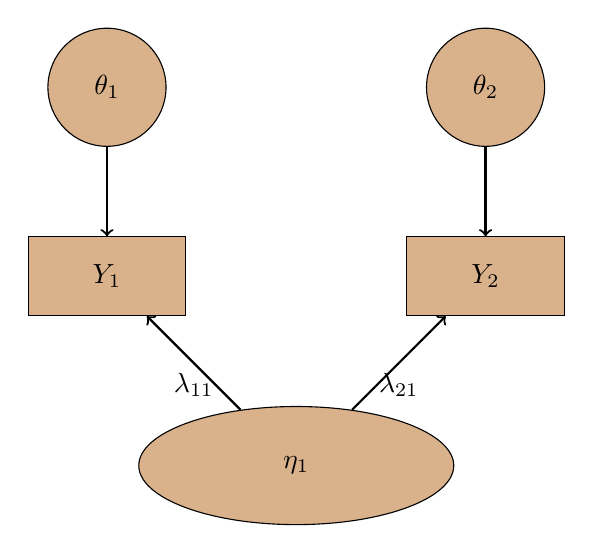
\begin{tikzpicture}[ factor/.style={draw,fill=brown!60, ellipse,minimum height=1.5cm, minimum width=4cm, node distance= {9cm}},
		latent/.style={draw, rectangle, minimum width=2cm, minimum height=1cm, fill=brown!60,node distance= {3.4cm}},
		residual/.style={draw,fill=brown!60,  circle, minimum width=1.5cm, minimum height=0.7cm, node distance= {2.4cm}}
		]
		\node [factor](x1) {$\eta_1$};
		\node [latent](y1) [above left of=x1] {$Y_1$};
		\node [latent](y2) [above right of=x1] {$Y_2$};
		\node [residual](e1) [above of=y1] {$\theta_1$};
		\node [residual](e2) [above of=y2] {$\theta_2$};
		\draw[thick, black, ->](x1) -- (y1) node[midway, below] {$\lambda_{11}$};
		\draw[thick, black, ->] (x1) -- (y2) node[midway, below] {$\lambda_{21}$};
		\draw[thick, black, ->] (e1) -- (y1);
		\draw[thick, black, ->] (e2) -- (y2);
	\end{tikzpicture}
	\label{Fig: Figure 3.2}
\end{figure}\\
\newpage
\noindent An example of just-identified model is:
\begin{figure}[h]
	\centering
	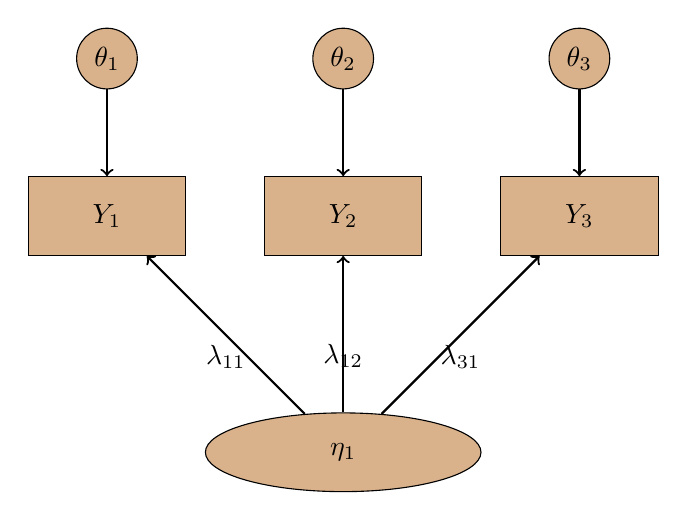
\begin{tikzpicture}[ factor/.style={draw,fill=brown!60, ellipse,minimum height=1cm, minimum width=3.5cm, node distance= {9cm}},
		latent/.style={draw, rectangle, minimum width=2cm, minimum height=1cm, fill=brown!60,node distance= {3cm}},
		residual/.style={draw,fill=brown!60,  circle, node distance= {2cm}}
		]
		\node [factor](x1) {$\eta_1$};
		
		\node [latent](y2) [above of=x1] {$Y_2$};
		\node [latent](y1) [left of=y2] {$Y_1$};
		
		\node [latent](y3) [right of =y2] {$Y_3$};
		
		\node [residual](e1) [above of=y1] {$\theta_1$};
		\node [residual](e2) [above of=y2] {$\theta_2$};
		
		\node [residual](e3) [above of=y3] {$\theta_3$};
		
		
		\draw[thick, black, ->](x1) -- (y1) node[midway, below] {$\lambda_{11}$};
		
		\draw[thick, black, ->] (x1) -- (y2) node[midway, below] {$\lambda_{12}$};
		
		\draw[thick, black, ->] (x1) -- (y3) node[midway, below] {$\lambda_{31}$};
		
		\draw[thick, black, ->] (e1) -- (y1);
		\draw[thick, black, ->] (e2) -- (y2);
		
		\draw[thick, black, ->] (e3) -- (y3);
		
	\end{tikzpicture}
	\label{Fig: Figure 3.3}
\end{figure}\\
\noindent Input matrix is :

$$B=\begin{pmatrix}
	& Y_1 & Y_2  & Y_3\\ 
	Y_1& \sigma_{11} &  & \\ 
	Y_2& \sigma_{21} & \sigma_{22} & \\ 
	Y_3&  \sigma_{31}&\sigma_{32}  & \sigma_{33}
\end{pmatrix}$$
We have 6 elements in the input matrix and 6 freely estimated model parameters.The df=6-6=0
\begin{figure}[h]
	\centering
	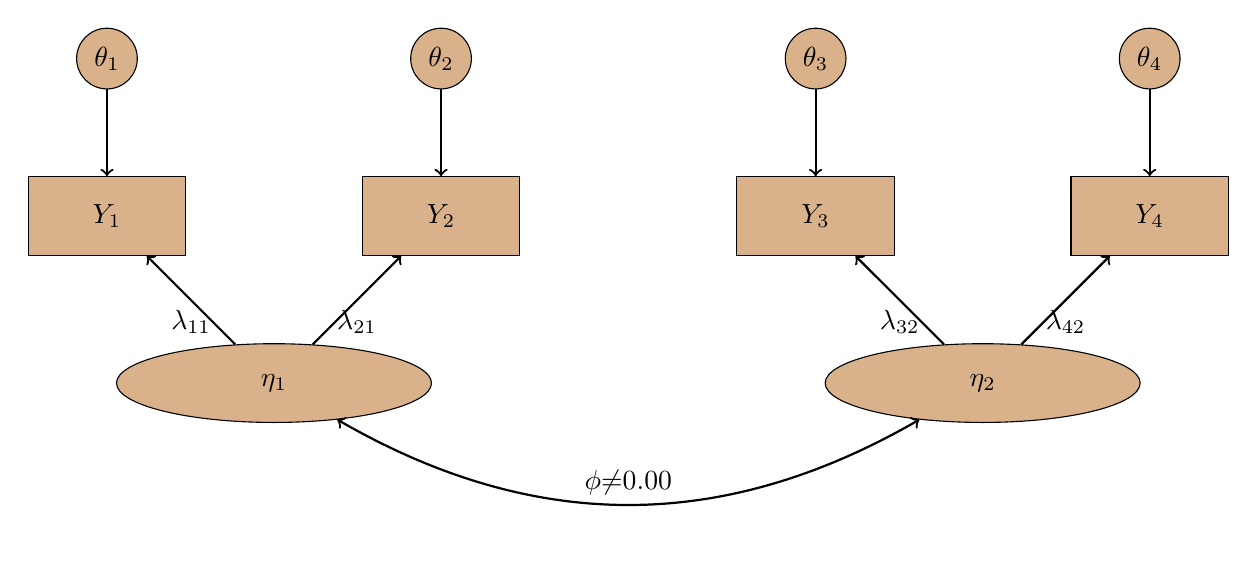
\begin{tikzpicture}[ factor/.style={draw,fill=brown!60, ellipse,minimum height=1cm, minimum width=4cm, node distance= {9cm}},
		latent/.style={draw, rectangle, minimum width=2cm, minimum height=1cm, fill=brown!60,node distance= {3cm}},
		residual/.style={draw,fill=brown!60,  circle, node distance= {2cm}}
		]
		\node [factor](x1) {$\eta_1$};
		\node [factor](x2)[right of =x1] {$\eta_2$};
		
		\node [latent](y1) [above left of=x1] {$Y_1$};
		\node [latent](y2) [above right of=x1] {$Y_2$};
		
		\node [latent](y3) [above left of =x2] {$Y_3$};
		\node [latent](y4) [above right of=x2] {$Y_4$};
		
		\node [residual](e1) [above of=y1] {$\theta_1$};
		\node [residual](e2) [above of=y2] {$\theta_2$};
		
		\node [residual](e3) [above of=y3] {$\theta_3$};
		\node [residual](e4) [above of=y4] {$\theta_4$};
		
		
		\draw[thick, black, ->](x1) -- (y1) node[midway, below] {$\lambda_{11}$};
		\draw[thick, black, ->] (x1) -- (y2) node[midway, below] {$\lambda_{21}$};
		
		\draw[thick, black, ->] (x2) -- (y3) node[midway, below] {$\lambda_{32}$};;
		\draw[thick, black, ->] (x2) -- (y4) node[midway, below] {$\lambda_{42}$};;
		
		\draw[thick, black, ->] (e1) -- (y1);
		\draw[thick, black, ->] (e2) -- (y2);
		
		\draw[thick, black, ->] (e3) -- (y3);
		\draw[thick, black, ->] (e4) -- (y4);
		
		\draw[thick, black, <->] (x1) edge[bend right=30] node[above] {$\phi$$\neq$0.00} (x2);
		
	\end{tikzpicture}
	\label{fig:Figure 3.4}
\end{figure}\\
\noindent Input matrix is :\\

$$C=\begin{pmatrix}
	& Y_1 & Y_2  & Y_3 & Y_4\\ 
	Y_1& \sigma_{11} &  & \\ 
	Y_2& \sigma_{21} & \sigma_{22} & \\ 
	Y_3&  \sigma_{31}&\sigma_{32}  & \sigma_{33} &\\
	Y_3&  \sigma_{31}&\sigma_{32}  & \sigma_{33} & \sigma_{44}
\end{pmatrix}$$

\noindent Note, df=10-9=1 Let b be the number of elements in the input matrix, and p be the
number of indicators included in the input matrix, then\\
$$b = p(p + 1)/2$$
\subsubsection{Descriptive Goodness Of Fit Indices}
One of the several models that can be used to estimate CFA models is ML (Maximum Likelyhood).\\
\noindent \textbf{\underline{Assumptions of ML}}

\begin{enumerate}
	\item The sample size is large (n $\geq$ 200)
	\item The indicators of the factors have been measured on continuous scale
	\item The distribution of the indicators is multivariate normal.
\end{enumerate}
Although the actual parameter estimates may not be affected,non-normality in ML analysis can result in biased standard errors and goodness of -fit statistics.
If non-normality is extreme, then ML will produce incorrect parameter estimates thus incase of non-normal continuous indicators it is better to use a different estimator such as ML with robust standard errors and chi-square (Satorra and Bentler, 1994).
There are a variety of goodness of fit statistics that provide a global desciptive summary of the ability of the model to reproduce the input covariance matrix. The classic goodness of fit is chi-square.
The idea is to test the hypothesis
$$H_0: S= \sum$$
$$H_1: S \neq \sum$$
The null hypothesis that the sample and model- implied variance – covariance matrices do not differ is retained.On the other hand a statistically significant chi square would lead to rejection of the null hypothesis meaning that the model estimates do not sufficiently reproduce the sample variances and covariances.


\noindent \textbf{\underline{NOTE}}\\
Under typical ML model estimation ${\chi}^2$ is defined as 
$$ {\chi}^2 = F_{ML}{(n-1)}$$ 
Except in M-plus where ${\chi}^2 = F_{ML}(n)$
If $\alpha$ is chosen as a level of significance then the critical value for the test is ${\chi}^2_\alpha (df)$. Where df = the number of known values - number of free parameters.\\
We reject the null hypothesis that $S= \sum$ at $\alpha$ level of significance if ${\chi}^2 = (n-1) F_{ML} > {\chi}^2_{\alpha (df)}$ and conclude that the model estimate do not sufficiently reproduce the sample variance and covariances (i.e., the model is not a good fit to the data. Otherwise we do not reject the null hypothesis.\\
In conclusion the model ${\chi}^2$ is the meaningful test only when we have an overidentified model so that there is a degrees of freedom left over after accounting for all the three parameters in our model.\\
The major drawback of chi square is that it is highly sensitive to sample size.
While chi square is routinely reported in CFA research, there are other fit indices which are used in the evaluation of model fit.These are;
\begin{enumerate}
	\item \textbf{Root Mean Square Error of Approximation}\\
	It is a population based index that relies on the noncentral chi square distribution, which is the distribution of the fitting function (e.g $F_{ML}$) when the fit of the model is not perfect.The model chi square and RMSEA belong to the class of indices called absolute fit indices.RMSEA is an error of approximation index because it asseses the extent to which a model fit reasonably well in the population.\\$$RMSEA= \sqrt {\frac{d}{df}}$$
	Where $d= {\chi}^2-{\frac{d_{df}}{n-1}}$\\
	The cut off criteria as defined in (Kline, 2016 pg. 274-276 ),\\
	\begin{itemize}
		\item $\leq 0.05$( close fit)
		\item Between 0.05 and 0.08 (reasonably approximate fit)
		\item $\geq 0.1$ ( poor fit)
	\end{itemize}
	The power of close fit is adversely affected by small sample size, but also by model saturation
	\item \textbf{Comparative Fit Index}\\
	It evaluates the fit of a user specified solution in relation to a more restricted,nested baseline model.\\The baseline model is a null or independent model in which the covariances among all input indicators are fixed to zero while $\delta_{users}$ is calculated from the target model.\\ The CFI has a range of possible values between 0 and 1 with values closer to one impying good model fit.\\
	Let $\delta = {\chi}^2-{df}$\\\\
	Then $CFI =\frac{\delta_{(Baseline)}-\delta_{(User)}}{\delta_{(Baseline)}}$
	
	\item \textbf{Tucker Lewis Index}\\
	It is referred to as the non-normed fit index in some programs.It has features that compensate for the effect of model complexity.It also includes a penalty function for adding freely estimated parameters that do not markedly improve the fit of the model.
	$$TLI =\frac{\frac{{\chi}^2_{(baseline)}}{df_{(baseline)}}- \frac{{\chi}^2_{(user)}}{df_(user)}}{\frac{{\chi}^2_{( baseline)}}{df_(baseline)} -1}$$.\\
\noindent Unlike CFI,TLI is non-normed which means that its values can fall outside the range of 0 to 1,values approaching one are interpreted in accord with good model fit.

\end{enumerate}

\subsection{Measurement Invariance (MI)}
\subsubsection{Conceptual introduction to measurement invariance}
Multiple-groups CFA is a technique that is used to see whether a theoretical model fits several groups simultaneously. That is, to test a hypothesis of whether a theoretical model fits well to the data across groups. We shall see if our CFA model fits the two gender(Male and Female).
Multi-Group CFA is therefore the standard procedure to which measurements invariance across groups is investigated.(Xu,2012) As noted by Timothy A. Brown CFA with multiple groups has many practical applications for example, measurement invariance evaluation addresses several issues that key to the Diagnostic and Statistical Manual-5 for mental health conditions, for instance, do the items of questionnaire measure the same construct (same factor structure) and evidence equivalent relationship to these constructs (equal factor loadings) in all subgroups of the population for whom the measure will be used. Does the questionnaire contain items that are biased against a particular subgroup, i.e., yield substantially higher or lower observed scores in a group at equivalent levels of the latent or true score? (UCLA,) Practical applications in mental health entail the cross-cultural validation of tests testing for equation of international tests (Wy, Li and Zumbo, 2007) and assessing the invariance of tests results across different subgroups e.g., the validity of somatic complaints in white and African American samples (Kline, 2003).\\

\noindent\textbf{MI definition:}\\

\noindent The statistical definition of MI is;(UCLA, ) \\
The observed random variable Y is said to be measurement invariant with respect to selection on G, 
if $$F(y|n,g)=F(y|n)$$ \\
$$ \forall (y,n, g)$$\\

\noindent in the sample space, where Y denotes an observed random variable with realization y; H denotes the latent variable (i.e. factor) with realization $\eta$ that is measurement by Y, or underlies Y; G denotes a random variable with realization g that functions as a selection of a sub-population from the parent population by application of a selection function
$$s(g), 0\leq s(g)\leq 1$$
\newpage
\noindent(Mellenburgh (1989), Meredith(1993), and Meredith and Millsup(1993) ).Thus, MI holds iff the probability of an observed score, given the true score and the group membership , is equal to the probability of that given only the true score. To fully address the question of “what constitutes MI?”, we consider a factor analysis model under means and covariance structure (MACS) modelling represented by a regression equation. (Kline, 2006 \& UCLA,) 

$$y_{ij}=\tau_j + \lambda_{j1}\eta_{1i}+\lambda_{j2}\eta_{2i}+...+\lambda_{jp}\eta_{pi}+\epsilon_{ij}$$

\noindent where;\\
\noindent $y_{ij}$ denotes the score of the i\textsubscript{th} person on the j\textsubscript{th} manifest variable(j=1,2,3,...J), (i=1,2, ..., N).\\
\noindent $\tau_j$ is the regresion intercept , i.e the $y_{ij}$  score at which the factors score is 0.\\
\noindent $\lambda_{jp}$ the regression slopes(coefficients), are the loadings from item j on factor p. \\
\noindent $\epsilon_{ij}$ is normally distributed random residuals or errors. \\
\noindent $\eta_{pi}$ represents factor(s) or latent variable(s), (p=1, 2, . . . , P).\\\\
\noindent Equality of these elements of the right-hand inside of equation (3.4.6) except for the residual term, i.e., equality in the model specification (number of factor and loading pattern), regression coefficient and regression intercept, ensures that the observed indicators have identical quantitative relationship with the latent variable(s) for each population of interest (Wu, Li, Zumbo, 2007). This the regression lines in equation above should be identical across all the groups for measurement invariance to hold. (Kline,2006).\\
\noindent Within the SEM framework different levels of measurement invariance may be defined as; 
\begin{itemize}
	\item Configural
	\item Weak
	\item Strong
	\item Strict Variance
\end{itemize}
\textbf{Configural invariance} implies that the number of latent variables and the pattern of loadings of latent variables on indicators are similar across the groups. \\
\textbf{Weak invariance}(also known as metric invariance) implies that the magnitude of the loadings is similar across the groups. This type of measurement invariance is required in order to meaningfully compare the relationships between latent variables across different groups. \\
\textbf{Strong invariance} (also known as scalar invariance) implies that not only the item loadings but also the item intercepts are similar across the groups. This form of measurement invariance implies that there are no systematic response biases and is required in order to meaningfully compare the means of latent variables across different groups (Chen, 2008).\\
\textbf{Strict invariance} implies that in addition to loadings and intercepts, the residual variances are similar across groups.\\\\
After having established measurement invariance, we may go on to test substantial hypotheses about the means and interrelations between latent constructs.
\subsubsection{Testing Measurement invariance}
\noindent Testing for measurement invariance consists of a series of model comparisons that define more and more stringent equality constraint(Bryne, 2009; Cheung \& Rensvold, 1999; Raju et al,2002; Vandenberg \& Lance, 2000).\\
Thus MCT-CFA involves a sequence of hypothesis tests of nested models beginning with the least constrained model, often the configural(Horn \& McAndle,1992), then progressively placing equality constraints on the parameters across groups. Hence, the subsequent test of measurement invariance is an argumentation of the parameter constraints of each proceeding hypothesis test. More demanding tests of measurement invariance will only proceed if less demanding level of invariance is satisfied. First, a baseline model is fit in which the loading pattern is similar in all groups but the magnitude of all parameter loadings, intercept, variances, etc. may vary. Configural invariance exists if the baseline model has a good fit and the same loadings are significant in all groups. Second, a weak invariance model in which the factor loadings are constrained to be equal is fit to the data and the fit of this model is compared to the baseline model. Weak invariance exists if the fit of the metric invariance model is not substantially worse than the fit of the baseline model. Third, a strong invariance model in which factor loadings and item intercepts are constrained to be equal is fit to the data and compared against the weak measurement invariance model. Again, strong invariance exists if the fit of the scalar invariance model is not substantially worse than the fit of the weak invariance model. Fourth, a strict invariance model in which factor loadings, intercepts, and residuals invariance are constrained to be equal is fit to the data and compared to the strong measurement invariance model. 

\subsubsection{Decision Rules for Invariance tests}

An open issue pertains the use of different decision rules for invariance (Wu et al,2007). The problem is that imposing equality constraints will always result in a decrease in fit because less degree of freedom are available (Hirschfeld and Von Brachel, 2014). \\
). Conventionally, the two -point decision about whether MG-CFA supports or rejects MI has solely relied upon the test of chi- squared difference between two nested models $\Delta{\chi}^2$, which itself follows a chi-square distribution with degree of freedom equal to the difference between those of the two nested models. The decision rule for whether MI holds relies upon whether the added constraints make a significant improvement to the model fit. A non- significant improvement in fit is considered as evidence for MI (Cheung \& Rensvold, 2002). \\

\noindent However, the $\Delta{\chi}^2$ test has been questioned (Brannick, 1995 \& Kelloway, 1995). In that the ${\chi}^2$= (N - 1) × minimum fitting function in single group CFA is a function of the sample size. \\
Therefore, (UCLA,) ${\chi}^2$ test is susceptible to sample size in the sense that it rejects the null hypothesis with too much power if the sample size is large. The chi-square difference is defined as:

$$\Delta{\chi}^2 = (n-1)[minimumfitingfunction_{aug} - minfittingfunction_{com}]$$

\noindent where;
Where “aug” denote the augmented model while “com” denotes more compact model. To accommodate the problems with sample size, a variety of fit indices have been developed such as comparative fit index (CFI, Bentler, 1990) and RMSEA (Steiger, 1989). \\
In line with measurement invariance, the inspection of changes in fit-indices, specifically the difference in comparative fit index $\Delta$(CFI), seem the most widely used and empirically the best supported criterion to define invariance (Chen, 2007, Cheung and Rensvold, 2002) at the present. \\
Most often a cut point of $\Delta$ $\leq$ 0.01, is chosen to decide whether a more constrained model, example, the weak-invariance model, shows a substantial decrease in model fit compared to a less constrained model, e.g. the baseline model. However, the sampling distributions of these fit indexes are unknown, hence, the formal hypothesis testing of the fit statistics cannot be conducted, (Wu, et al, 2007).
\subsubsection{Results of Measurement of invariance}

A scale is said to have measurement invariance across groups if subjects with identical levels of the latent construct have the same expected raw-score on the measure (Drasgow and Kanfer, 1985). As such, the level of measurement invariance a scale exhibits has very important implication for the interpretation of differences. If measurement invariance has been established for a measure, observed mean differences can be attributed to differences in underlying constructs between the groups. If, however, one cannot assume a stable relation between underlying construct and scale score, observed mean differences may be either due to differences in underlying constructs, or due to the different relations between latent constructs and scores. 
There are currently two approaches to test for invariance; structural equation modelling, and item response theory (Raju, Laffitte and Byrne, 2002; Reise, Widaman and Pugh, 1993). Structural equation modelling (SEM) lends itself naturally to investigate the invariance of the relations between underlying constructs (latent variables) and observed responses, since these relations are explicitly modelled.
\newpage
\subsection{Sources of Data}
The data used in this project is a dataset collected from different devices, accessible through the kobo Toolbox interface.It consists of depression severity test scores of persons between the age of 18 and 40.This data frame consists of 230 observations of 12 variables.
\subsubsection{Variable description}
$x1<-$Trouble falling or staying asleep or sleeping too much.\\
$x2<-$Feeling down, depressed or hopeless.\\
$x3<-$Felt that i had nothing to look forward to.\\
$x4<-$Feeling tired or having little energy.\\
$x5<-$Feeling bad about yourself -or that you are a failure or have let yourself or your family down.\\
$x6<-$I felt unhappy.\\
$x7<-$Moving or speaking so slowly that other people could have noticed?\\
$x8<-$Poor appetite or overeating\\
$x9<-$Thoughts that you would be better off dead or hurting yourself in some way.

\subsubsection{The Path Diagram}
The path diagram can assist us in understanding our CFA model because it is asymbolic one-to-one visualization of the measurement model and the
model-implied covariance. Circles represent latent variables, squares represent observed indicators and one-way arrows represent paths.
\begin{figure}[ht]
	\centering
		\begin{adjustbox}{height=15cm}
		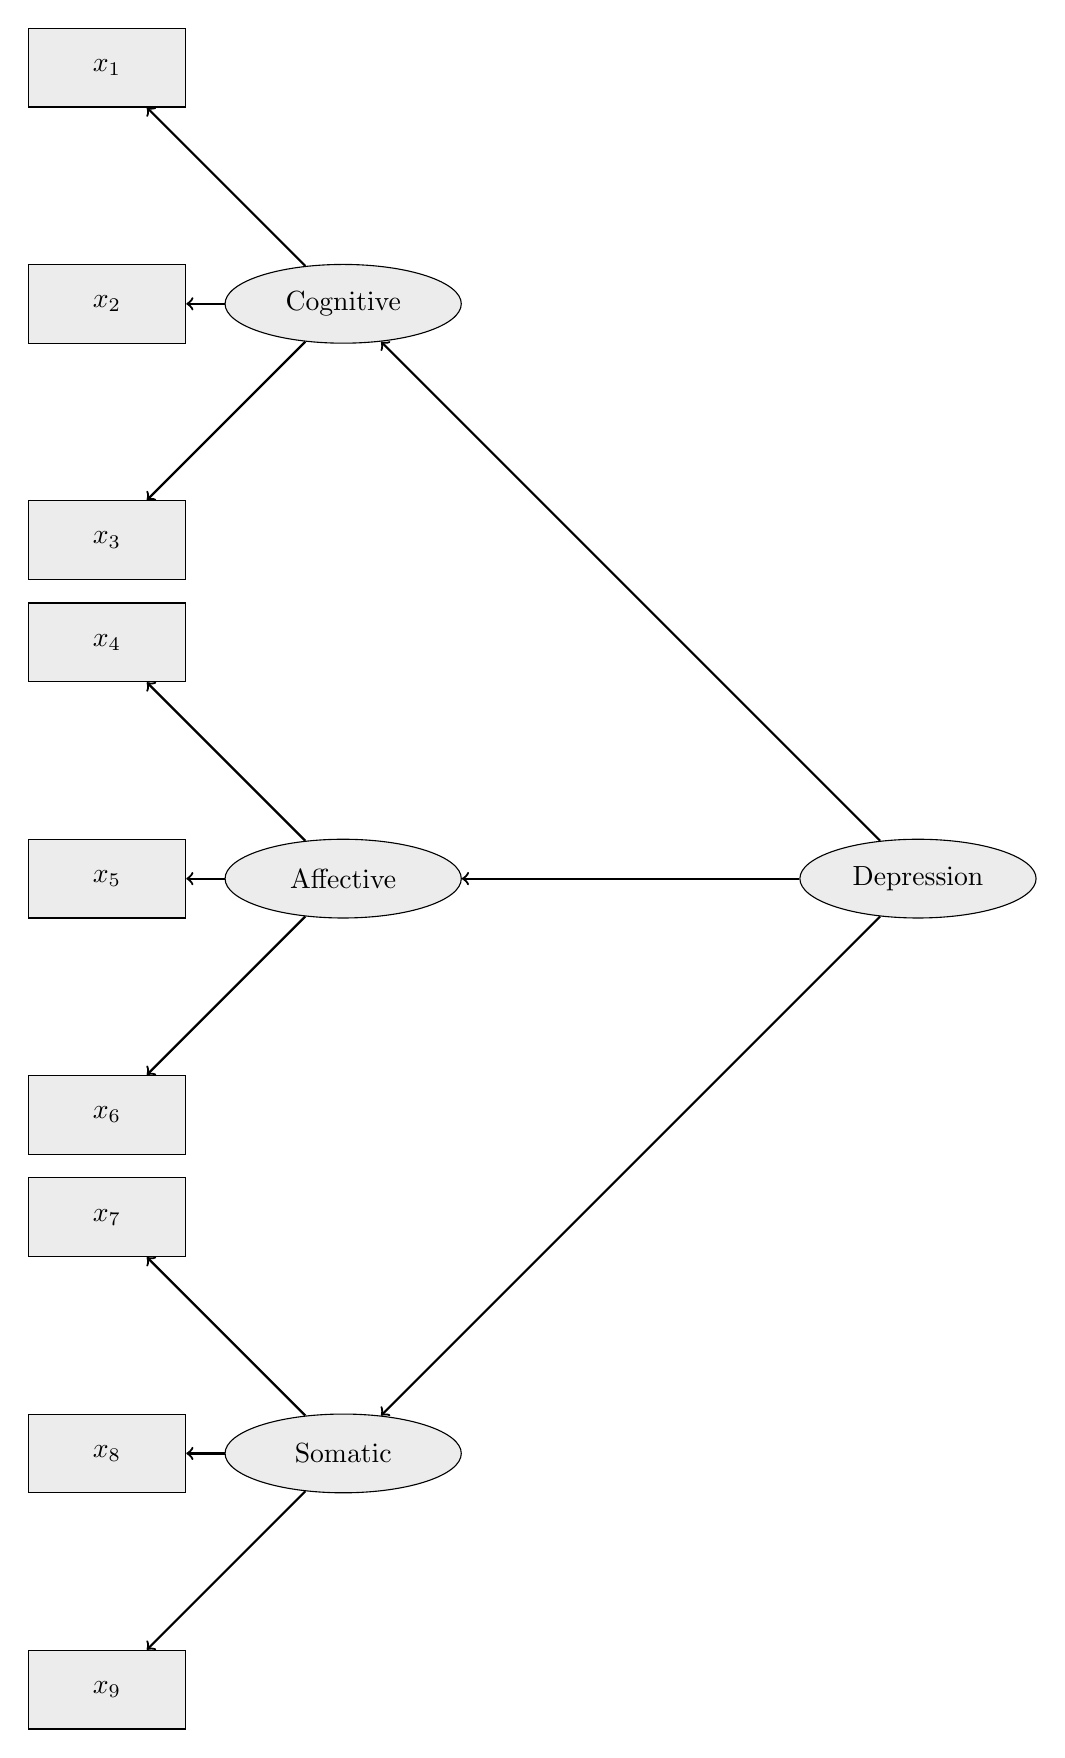
\begin{tikzpicture}[ latent/.style={draw,fill=lightgray!30, ellipse,minimum height=1cm, minimum width=3cm, node distance= {7.3cm}},
			indicator/.style={draw, rectangle, minimum width=2cm, minimum height=1cm, fill=lightgray!30,node distance= {3cm}},
			]
			\node [latent](x0) {Depression};
			
			\node [latent](x2)[left of =x0] {Affective};
			\node [latent](x1)[above of =x2] {Cognitive};
			\node [latent](x3)[below of =x2]{Somatic};
			
			\node [indicator](y2) [left of=x1] {$x_2$};
			\node [indicator](y1) [above of=y2] {$x_1$};
			\node [indicator](y3) [below of=y2] {$x_3$};
			
			\node [indicator](y5) [left of =x2] {$x_5$};
			\node [indicator](y4) [above of=y5] {$x_4$};
			\node [indicator](y6) [below of =y5] {$x_6$};
			
			\node [indicator](y8) [left of =x3] {$x_8$};
			\node [indicator](y7) [above of=y8] {$x_7$};
			\node [indicator](y9) [below of =y8] {$x_9$};
			
			\draw[thick, black, ->](x0) -- (x1);
			\draw[thick, black, ->] (x0) -- (x2);
			\draw[thick, black, ->] (x0) -- (x3);
			
			\draw[thick, black, ->] (x1) -- (y1);
			\draw[thick, black, ->] (x1) -- (y2);
			\draw[thick, black, ->] (x1) -- (y3);
			
			\draw[thick, black, ->] (x2) -- (y4);
			\draw[thick, black, ->] (x2) -- (y5);
			\draw[thick, black, ->] (x2) -- (y6);
			
			\draw[thick, black, ->] (x3) -- (y7);
			\draw[thick, black, ->] (x3) -- (y8);
			\draw[thick, black, ->] (x3) -- (y9);
			
		\end{tikzpicture}
		\end{adjustbox}
	\caption{Depression severity data CFA model}
\end{figure}

\newpage
\section*{References}
\indent Brown T. A.  and Moore M.T. (2012), Confirmatory Factor Analysis, \emph{Handbook of Structural Equation Modelling}, pg no 361 -379.\\
\indent Brown T. A., Confirmatory Factor Analysis for Applied Research, \emph{The Guilford Press},2015.\\
\indent Donna L. M., Sherry S. C., Kevin C. and Amit S.(2017), Results support blended learning using SMART as a strategy to increase access to resiliency training for nursing staff, \emph{The Journal of Nursing Administration},Vol. 47(8), pp. 391-395.\\
\indent Gagan J., Anuja R., Venkatesh H., Shawn Y., Omar D. and Carol L., Patient-reported Depression Severity Measured by the PHQ-9 and Impact on Work Productivity, \emph{Journal of Occupational and Environmental Medicine}, March 2013, Vol.55 (3), pp. 252-258.\\
\indent Greg J.S., Stephanie L.T. and Kirsten T.(2020), Mindfulness-based Stress Reduction (MBSR) Reduces Anxiety, Depression and Suicidal Ideation in Veterans, \emph{Medical Care and Building the Evidence Base for Complementary and Integrative Medicine Use among Veterans and Military Personnel}, (December 2014), Vol.52(12), pp. S19-S24.\\
\indent Johnson R.A. and Wichern D.W.,Applied Multivariate Statistical Analysis, \emph{ Pearson Education, Inc.}, 2007.\\
\indent Kline R.B., Principles and Practice of Structural Equation Modeling, \emph{ The Guilford Press}, 2016.\\
\indent Leung D.Y.P., Chiang V.C.L., Mak Y.W., Loke A.Y., Leung S.F.(2020), Measurement Invariances of the PHQ-9 Across Gender and Age Groups in Chinese Adolescents, \emph{Asia-Pacific Psychiatry},Vol.12, pg no.1-6.\\

\indent Levis B., Benedetti A. and Thombs B.D. (2019), Accuracy of Patient Health Questionnaire-9 (PHQ-9) for Screening to Detect Major Depression,\emph{British Medical Journal}, Vol. 365(1476), Pages 1-10.\\
\indent Levis B., Sun Y., He C., Wu Y., Krishnan A., Bhandari P.M., Neupane D. ,Imran M. ,Brehaut E. ,Negeri Z. ,Fischer F.H. ,Benedetti A. and Thombs B.D. , Accuracy of the PHQ-2 Alone and in Combination with the PHQ- 9 for Screening to Detect Major, \emph{Depression,Systematic Review and Meta Analysis}, Vol.323(22), pg no.2290-2300\\
\indent Martin A. ,Sanderson K. and Cocker F. (2009), Meta Analysis of the Effects of Health Production Intervention in the Workplace on Depression and Anxiety symptoms, \emph{Scandinavian Journal of Work}, Environment and Health, Vol.35 (1), pg no. 7 – 18\\
\indent Sharon S. L. and Salene M.W. J., workplace culture of health was negatively correlated with anxiety and depression,\emph{Journal of Occupational and Environmental Medicine}, November 2016, Vol. 58(11), pp. 1144-1149.\\
\indent UCLA. Confirmatory factor analysis (cfa) in r with lavaan, 
\href{https://stats.oarc.ucla.edu/r/seminars/rcfa/}{Accessed April 2023} \\
\indent Xu K. (2012). Multiple group measurement: invariance analysis in lavaan, \emph{Cambridge Mass}, 37.\\

\end{document}

